\chapter{Histoire thermique, dernière diffusion et soupe primordiale}

\lectureoverview{L’histoire de l’expansion de l’Univers est aussi une histoire thermique. Nous commencerons par définir la température à partir de l’équilibre, et l’équilibre à partir des diffusions. Un gaz de photons acquiert le spectre de Planck tant que des charges libres le maintiennent à l’équilibre thermique ; lorsque les électrons se lient aux protons, le rayonnement se découple, mais conserve sa forme de corps noir à mesure que toutes ses longueurs d’onde s’étirent avec le facteur d’échelle. L’immense rapport entre le nombre de photons et celui de particules de matière explique alors pourquoi la recombinaison se produit bien en dessous de la température d’ionisation de l’hydrogène. En remontant encore le temps, nous traverserons la dernière diffusion, l’égalité matière--rayonnement, l’équilibre des paires électron--positron, puis le faible excès de matière--antimatière qui subsiste après l’annihilation.}

\section{De l’ajustement des modèles à l’histoire thermique}

Un modèle cosmologique est défini, au minimum, par l’histoire du facteur d’échelle et par une géométrie spatiale,
\begin{equation}
a(t),
\qquad
k\in\{+1,0,-1\}.
\end{equation}
La méthode pratique consiste à choisir le modèle, à calculer ses prédictions, à les comparer aux données, puis à ajuster les paramètres. Il est possible d’inverser directement le raisonnement à partir des données, mais cette approche est souvent moins transparente.

Il est difficile de déterminer la courbure à partir de sources relativement proches. De même que la courbure de la Terre n’apporte qu’une faible correction sur une courte distance, la courbure spatiale a peu d’effet lorsque la distance cosmologique considérée est trop faible. C’est à la fois un inconvénient et un avantage : les relevés ordinaires de sources ne déterminent pas précisément \(k\), mais une incertitude modérée sur \(k\) n’empêche pas de reconstituer utilement l’histoire de l’expansion.

Deux grandes familles d’observables fournissent l’essentiel de l’information. Les chandelles standard donnent la luminosité en fonction du décalage vers le rouge, tandis que les relevés de sources donnent le nombre d’objets dans un intervalle de décalage vers le rouge. Les ajustements qui en résultent favorisent une histoire de l’expansion comportant une contribution importante de l’énergie du vide. Pour obtenir une information précise sur la courbure, il faut le bras de levier géométrique bien plus long fourni par le fond diffus cosmologique.

Changeons maintenant de question. Au lieu de demander seulement comment \(a(t)\) évolue, demandons-nous comment évolue la température de l’Univers. Cette question en appelle une plus élémentaire : dans quelles conditions un système possède-t-il une température ?

\section{Quand l’Univers a une température}

La température est une propriété de l’équilibre thermique. Un ensemble de particules tend vers l’équilibre par des collisions, qui doivent se produire plus rapidement que les changements de l’environnement macroscopique. Dans un Univers en expansion, la comparaison pertinente est
\begin{equation}
\tau_{\rm scatt}\ll H^{-1},
\label{eq:c07-equilibrium-condition}
\end{equation}
où \(\tau_{\rm scatt}\) est un temps caractéristique de diffusion et \(H^{-1}\) le temps caractéristique de l’expansion. Lorsque cette inégalité n’est plus vérifiée, l’Univers évolue plus vite que les collisions ne peuvent rétablir l’équilibre.

Considérons une boîte parfaitement réfléchissante. Faisons-y entrer une impulsion laser, refermons l’ouverture et supposons que la boîte ne contienne que des photons. L’impulsion rebondit indéfiniment, mais les photons ordinaires de basse énergie diffusent les uns sur les autres avec une extrême faiblesse. La réflexion, à elle seule, ne redistribue pas leur énergie selon un spectre thermique. Un gaz de photons ne se thermalise donc pas simplement parce qu’il est confiné.

La présence de particules chargées libres change la situation. Une onde électromagnétique accélère un électron ; la charge accélérée réémet du rayonnement, de sorte que les photons diffusent efficacement. Si les électrons et les protons libres sont assez nombreux, les diffusions répétées redistribuent l’énergie entre les trois espèces jusqu’à ce qu’elles forment une même soupe thermique à température commune.

À grande échelle, l’Univers est électriquement neutre. Dans le décompte le plus simple,
\begin{equation}
n_{e^-}=n_p,
\label{eq:c07-neutrality}
\end{equation}
car les charges de l’électron et du proton ont la même valeur absolue et des signes opposés. Cette équation exprime la neutralité ; elle n’explique ni pourquoi la charge totale est neutre, ni pourquoi les valeurs absolues des deux charges sont égales. Ce sont là des faits plus profonds de la physique des particules.

La distinction entre un plasma et un gaz neutre est déterminante. Les électrons libres diffusent efficacement le rayonnement. Dès qu’ils se lient aux protons pour former de l’hydrogène neutre, les champs électriques dominants se compensent à longue distance et la diffusion devient beaucoup moins efficace. À la faible densité de l’Univers actuel, la matière neutre ne peut pas mettre les photons du fond en équilibre au cours d’une durée égale à l’âge de l’Univers.

À une température assez élevée, les collisions énergétiques ionisent sans cesse l’hydrogène et entretiennent une population importante de charges libres. Les électrons, les protons et les photons sont alors à la même température. Quand le système se refroidit, les atomes subsistent, la densité d’électrons libres s’effondre et l’équilibre commun se perd. Les températures attribuées ensuite à la matière et au rayonnement ne sont pas nécessairement égales.

\begin{classroomqa}
\audiencequestion{Si le fond diffus micro-onde a une température proche de \(3\,\mathrm{K}\), est-ce la température de tout l’Univers aujourd’hui ?}
\lecturerresponse{Non. On peut caractériser le spectre des photons par une température de corps noir, mais la matière actuelle n’est pas en équilibre avec ces photons. Les différentes composantes ont des températures cinétiques ou effectives différentes ; il n’existe donc pas aujourd’hui de température thermodynamique globale unique.}
\end{classroomqa}

\section{Rayonnement thermique et transition quantique}

Un champ de rayonnement à l’équilibre contient un spectre de longueurs d’onde et de fréquences reliées par
\begin{equation}
\nu\lambda=c.
\end{equation}
Pour ne pas confondre la luminance avec la densité d’énergie, notons \(u_\nu(T)\) l’énergie par unité de volume et par unité de fréquence :
\begin{equation}
dE=u_\nu(T)\,dV\,d\nu.
\label{eq:c07-spectral-density}
\end{equation}
Ainsi, \(u_\nu\) a pour dimensions l’énergie divisée par le volume et par la fréquence.

La température est elle-même une échelle d’énergie. Les unités historiques de température masquent ce fait ; la constante de Boltzmann assure la conversion :
\begin{equation}
E_{\rm thermal}\sim k_B T.
\end{equation}
On peut poser \(k_B=1\) en unités naturelles, mais la conserver permet de distinguer visiblement les kelvins de l’énergie.

Avant la mécanique quantique, l’analyse dimensionnelle fondée sur \(k_BT\), \(\nu\) et \(c\) donne la densité spectrale d’énergie de Rayleigh--Jeans,
\begin{equation}
u_\nu^{\rm RJ}(T)=\frac{8\pi\nu^2}{c^3}k_BT.
\label{eq:c07-rayleigh-jeans}
\end{equation}
Le facteur numérique dépend du dénombrement des modes électromagnétiques, mais le comportement classique essentiel est \(u_\nu\propto T\nu^2\). Cette quantité croît sans limite lorsque la fréquence augmente, ce qui conduit à prédire
\begin{equation}
\int_0^\infty u_\nu^{\rm RJ}\,d\nu=\infty.
\end{equation}
Ce résultat impossible est la catastrophe ultraviolette. Le spectre mesuré croît au contraire, atteint un maximum, puis décroît assez rapidement pour que son énergie totale soit finie.

La constante de Planck introduit l’échelle quantique manquante. Pour la densité spectrale d’énergie définie dans l’équation~\eqref{eq:c07-spectral-density}, la loi de Planck s’écrit
\begin{equation}
u_\nu(T)
=
\frac{8\pi h\nu^3}{c^3}
\frac{1}{e^{h\nu/(k_BT)}-1}.
\label{eq:c07-planck}
\end{equation}
L’exposant dépend du rapport sans dimension
\begin{equation}
x=\frac{h\nu}{k_BT},
\end{equation}
car \(E_\gamma=h\nu\) et \(k_BT\) sont tous deux des énergies.

À basse fréquence, \(x\ll1\), et
\begin{equation}
e^x-1=x+O(x^2).
\end{equation}
En substituant dans l’équation~\eqref{eq:c07-planck}, on obtient
\begin{align}
u_\nu(T)
&\simeq
\frac{8\pi h\nu^3}{c^3}
\frac{k_BT}{h\nu}
\\
&=
\frac{8\pi\nu^2}{c^3}k_BT,
\end{align}
La physique classique est ainsi retrouvée dans son domaine de validité, celui des basses fréquences. À haute fréquence, \(x\gg1\), l’exponentielle domine et supprime le spectre. La transition se produit lorsque
\begin{equation}
\frac{h\nu}{k_BT}\sim1.
\label{eq:c07-crossover}
\end{equation}
C’est là que la décroissance quantique prend le relais de la croissance classique.

\begin{figure}[htbp]
\centering
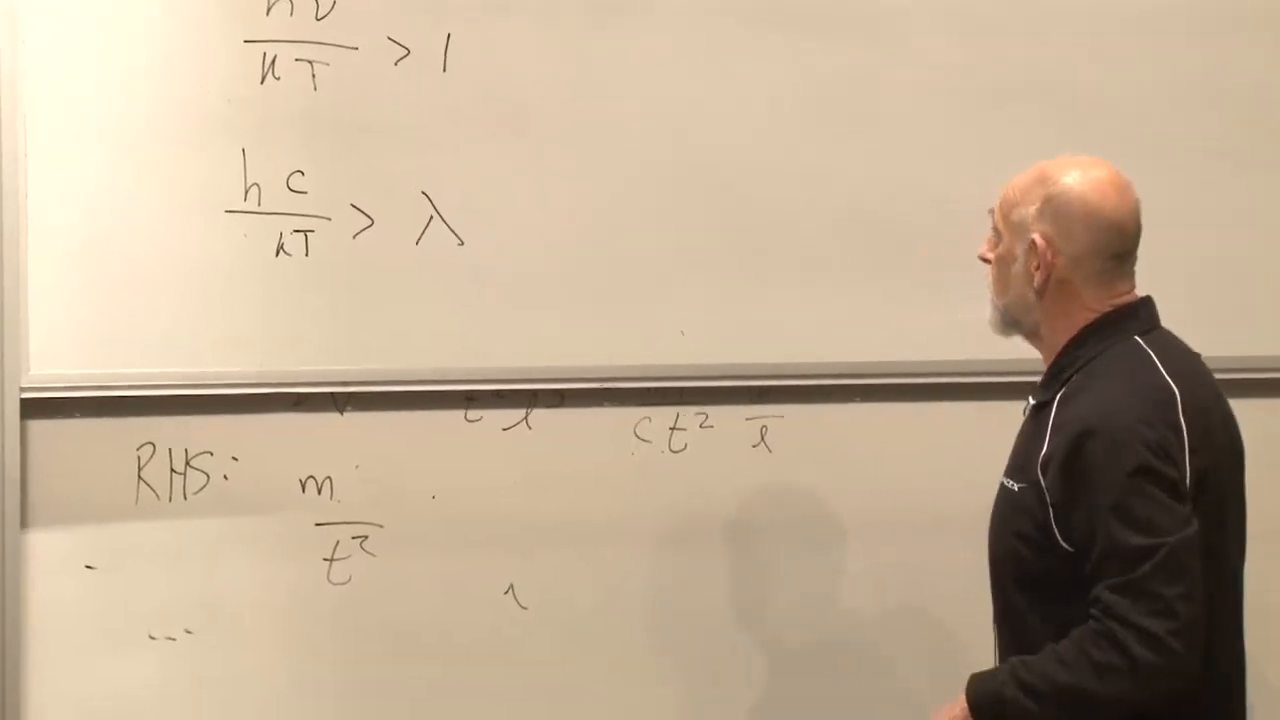
\includegraphics[width=0.82\textwidth]{lecture_07_figure_02.png}
\caption{La transition thermique au tableau. L’expression tronquée en haut est \(h\nu/(kT)>1\), et l’expression du bas, bien visible, est \(hc/(kT)>\lambda\). Les traces peu lisibles sur le tableau inférieur ne sont pas utilisées comme preuve de l’équation.}
\label{fig:c07-thermal-board}
\lectureframe{00:44:42.840}
\end{figure}

En utilisant \(\nu=c/\lambda\), la transition définit une longueur d’onde thermique d’ordre de grandeur
\begin{equation}
\boxed{\lambda_{\rm th}\sim\frac{hc}{k_BT}}.
\label{eq:c07-thermal-wavelength}
\end{equation}
Les longueurs d’onde plus courtes se trouvent dans la queue à décroissance exponentielle ; la majeure partie de la puissance est portée par des longueurs d’onde de cet ordre, à un facteur numérique près qui dépend de la représentation du spectre par unité de fréquence ou par unité de longueur d’onde.

\begin{classroomqa}
\audiencequestion{Planck a-t-il obtenu ce spectre à partir du modèle de plasma électron--proton utilisé ici ?}
\lecturerresponse{Non. Il a combiné des données spectrales empiriques avec la loi de déplacement de Wien, qui montrait déjà que la longueur d’onde au maximum varie en raison inverse de la température. Cette loi d’échelle a révélé l’existence d’une nouvelle constante \(h\). Planck a relié le résultat aux oscillateurs présents dans les parois matérielles ; l’interprétation quantique complète du champ de rayonnement est venue plus tard. \lecturetimestamp{00:37:06--00:39:25}}
\end{classroomqa}

\begin{classroomqa}
\audiencequestion{Pourquoi la vérification dimensionnelle semblait-elle omettre une puissance de \(c\) ?}
\lecturerresponse{La quantité d’abord appelée intensité était définie comme l’énergie par unité de volume et par unité de fréquence, tandis que la formule familière comportant \(2h\nu^3/c^2\) correspond à la luminance spectrale par unité de surface et d’angle solide. La densité spectrale d’énergie comporte \(c^{-3}\) et un facteur angulaire, comme dans l’équation~\eqref{eq:c07-planck}. Cette correction modifie la convention de normalisation, mais pas le rapport sans dimension \(h\nu/(k_BT)\) ni la longueur d’onde thermique. \lecturetimestamp{00:39:33--00:44:51}}
\end{classroomqa}

À un facteur de normalisation près, le spectre de Planck a une forme universelle. L’équation~\eqref{eq:c07-planck} peut s’écrire
\begin{equation}
u_\nu(T)=T^3\,F\!\left(\frac{\nu}{T}\right),
\label{eq:c07-scaling-form}
\end{equation}
les constantes étant incorporées dans \(F\). Augmenter \(T\) redimensionne l’axe des fréquences et la hauteur globale ; on retrouve la même courbe sans dimension. Dans la représentation en longueur d’onde, augmenter la température resserre le spectre vers les longueurs d’onde plus courtes.

\begin{figure}[htbp]
\centering
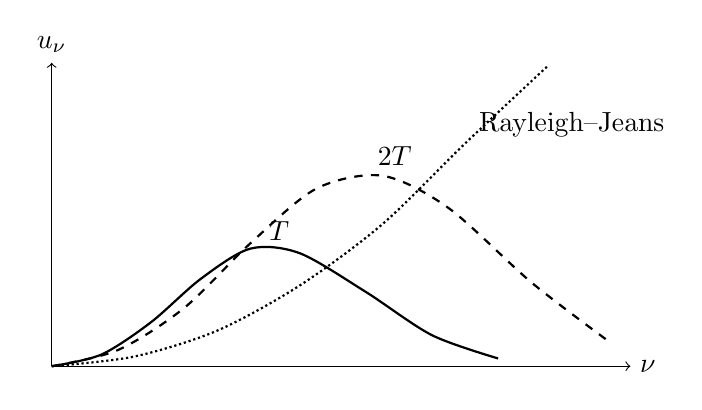
\begin{tikzpicture}[x=1.05cm,y=0.82cm]
\draw[->] (0,0)--(7.0,0) node[right] {\(\nu\)};
\draw[->] (0,0)--(0,4.7) node[above] {\(u_\nu\)};
\draw[densely dotted,thick] plot[smooth] coordinates
  {(0,0) (1,0.15) (2,0.55) (3,1.25) (4,2.20) (5,3.45) (6,4.65)};
\draw[thick] plot[smooth] coordinates
  {(0,0) (0.6,0.18) (1.2,0.68) (1.8,1.35) (2.4,1.82) (3.0,1.75) (3.8,1.15) (4.6,0.48) (5.4,0.12)};
\draw[thick,dashed] plot[smooth] coordinates
  {(0,0) (0.8,0.25) (1.6,0.90) (2.4,1.90) (3.2,2.75) (4.0,2.95) (4.8,2.45) (5.8,1.30) (6.7,0.42)};
\node[anchor=west] at (5.05,3.75) {Rayleigh--Jeans};
\node at (2.75,2.10) {\(T\)};
\node at (4.15,3.25) {\(2T\)};
\end{tikzpicture}
\caption{Le spectre classique croît sans limite, tandis que les spectres de Planck atteignent un maximum puis décroissent. L’augmentation de la température déplace la fréquence caractéristique vers les hautes fréquences et préserve la forme sans dimension.}
\label{fig:c07-planck-redraw}
\end{figure}

L’immense majorité des photons de l’Univers actuel appartient au fond diffus micro-onde et a une longueur d’onde caractéristique de l’ordre du millimètre. L’équation~\eqref{eq:c07-thermal-wavelength} associe cette longueur d’onde à quelques kelvins, arrondis ici conventionnellement à \(3\,\mathrm{K}\). Une longueur d’onde, à elle seule, ne fournirait qu’une estimation grossière. L’indice plus probant est que les mesures effectuées à de nombreuses fréquences suivent la courbe complète du corps noir avec une très grande précision.

\begin{classroomqa}
\audiencequestion{Quel volume occupe un photon du fond diffus micro-onde ?}
\lecturerresponse{Un photon n’a pas de taille définie par une frontière universelle. On peut le préparer sous la forme d’un paquet d’ondes dont l’étendue spatiale dépend de l’état, tandis que sa longueur d’onde fixe l’échelle de ses oscillations. Pour le fond thermique, la longueur d’onde caractéristique et une échelle naturelle du paquet d’ondes sont toutes deux de l’ordre du millimètre, mais aucune ne doit être confondue avec le rayon d’un petit objet classique. \lecturetimestamp{00:57:16--00:59:05}}
\end{classroomqa}

\section{L’expansion préserve la forme du corps noir}

Considérons d’abord une boîte chaude contenant de l’hydrogène ionisé et du rayonnement à l’équilibre. À mesure que la boîte se dilate, son contenu fournit du travail, la densité d’énergie diminue et la température baisse. À terme, les électrons et les protons restent liés sous forme d’atomes neutres. La formation des atomes est appelée \emph{recombinaison} ; la perte de l’efficacité de la diffusion des photons--matière est appelée \emph{découplage}. Ces deux processus sont étroitement liés, mais désignent des événements physiques différents.

Après le découplage, la matière et le rayonnement ne partagent plus une température commune. Pourtant, le spectre des photons conserve sa forme de Planck. Toutes les longueurs d’onde qui se propagent librement s’étirent selon le même facteur d’expansion,
\begin{equation}
\lambda\propto a,
\qquad
\nu\propto a^{-1}.
\end{equation}
Puisque la courbe de Planck dépend de \(\nu/T\), ce décalage uniforme vers le rouge équivaut à attribuer au rayonnement une température
\begin{equation}
\boxed{T_\gamma\propto a^{-1}.}
\label{eq:c07-temperature-scaling}
\end{equation}
L’expansion préserve donc la forme du spectre même si aucune collision ne la reconstitue en permanence. La matière suit ensuite sa propre évolution thermique.

Le fond diffus micro-onde observé est donc un vestige d’une distribution d’équilibre. Sa forme de corps noir s’est établie lorsque les charges libres diffusaient efficacement le rayonnement ; elle a ensuite été préservée par le décalage cosmologique uniforme vers le rouge. Il existe aussi la lumière des étoiles, les rayons gamma et d’autres sources plus tardives, mais leur nombre est faible comparé à celui des photons fossiles, et leurs origines astrophysiques sont identifiables.

\begin{classroomqa}
\audiencequestion{Comment le rayonnement peut-il rester un corps noir alors qu’il n’est plus en équilibre avec la matière ?}
\lecturerresponse{Les collisions sont nécessaires pour créer le spectre d’équilibre, mais pas pour le préserver lors d’une expansion parfaitement uniforme. Multiplier toutes les longueurs d’onde par le même facteur transforme un spectre de Planck en un autre, de température plus basse. Les photons cessent de partager la température de la matière, tout en conservant leur propre température de corps noir.}
\end{classroomqa}

\section{Pourquoi la recombinaison se produit si tard}

La longueur d’onde aujourd’hui et celle au découplage sont reliées par
\begin{equation}
\frac{\lambda_0}{\lambda_{\rm dec}}
=
\frac{a_0}{a_{\rm dec}}
=
\frac{T_{\rm dec}}{T_0}.
\label{eq:c07-decoupling-ratio}
\end{equation}
Le découplage n’est pas mathématiquement instantané, mais il est assez bref par rapport à l’évolution ultérieure pour qu’on puisse lui attribuer un facteur d’échelle et une température caractéristiques. Ici, \(T_0\) désigne la température du fond diffus cosmologique, et non la température cinétique de la matière intergalactique.

L’énergie d’ionisation de l’hydrogène dans son état fondamental est
\begin{equation}
\chi_H=13.6\,\mathrm{eV}.
\end{equation}
Une première estimation consisterait à poser \(k_BT\sim\chi_H\), de sorte qu’un photon typique puisse ioniser un atome. Cette estimation donne une température bien trop élevée, car un spectre thermique comporte une queue de haute énergie et l’Univers contient un nombre immense de photons.

\begin{figure}[htbp]
\centering
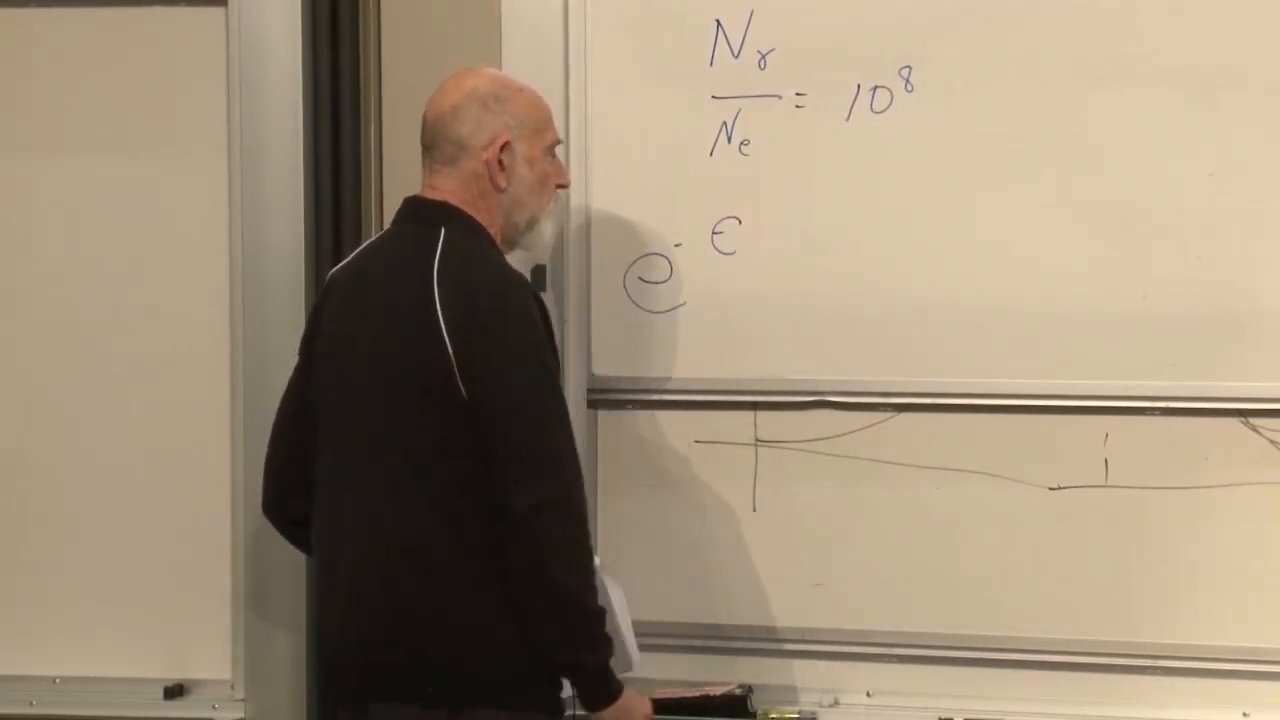
\includegraphics[width=0.82\textwidth]{lecture_07_figure_03.png}
\caption{Le tableau introduit le rapport d’abondance observé \(N_\gamma/N_e=10^8\) et le symbole de l’énergie des photons \(\epsilon\). Seul le début de l’exponentielle est visible ; le facteur de Boltzmann complet découle du raisonnement exposé oralement.}
\label{fig:c07-boltzmann-board}
\lectureframe{01:06:10.631}
\end{figure}

Le rapport d’abondance arrondi utilisé ici est
\begin{equation}
\frac{N_\gamma}{N_e}\sim10^8.
\label{eq:c07-photon-electron-ratio}
\end{equation}
On le déduit en comparant la densité mesurée des photons du fond diffus cosmologique à la quantité de matière ordinaire. Pour une énergie de photon \(\epsilon\), la queue de haute énergie suit une loi de Boltzmann de la forme
\begin{equation}
P(\epsilon)\propto e^{-\epsilon/(k_BT)}.
\end{equation}
On estime donc le nombre de photons ionisants disponibles par atome par
\begin{equation}
10^8 e^{-\chi_H/(k_BT)}.
\end{equation}
L’ionisation reste efficace jusqu’à ce que cette quantité tombe à un ordre de grandeur de l’unité.

En prenant les logarithmes, on obtient
\begin{equation}
\frac{\chi_H}{k_BT}
\sim
\ln 10^8
\simeq18.4,
\end{equation}
ou, à la précision visée,
\begin{equation}
k_BT\sim\frac{\chi_H}{20}.
\label{eq:c07-tail-estimate}
\end{equation}
Le photon caractéristique peut être très en dessous du seuil, car un seul photon ionisant de la queue suffit pour chaque atome.

\begin{classroomqa}
\audiencequestion{L’estimation fondée sur la queue compte-t-elle les photons exactement au seuil ou tous ceux qui le dépassent ?}
\lecturerresponse{Elle compte les photons au seuil et au-dessus. Comme la queue décroît exponentiellement, la majeure partie de cette intégrale provient des énergies proches de \(\chi_H\) ; l’estimation exponentielle simple donne donc le bon ordre de grandeur. \lecturetimestamp{01:08:39--01:08:54}}
\end{classroomqa}

\begin{classroomqa}
\audiencequestion{Le rapport \(N_\gamma/N_e\) était-il également de l’ordre de \(10^8\) au découplage ?}
\lecturerresponse{Dans l’approximation utilisée ici, oui. Depuis le découplage jusqu’aux époques nettement plus chaudes, l’expansion dilue les deux populations selon le même facteur de volume et ne crée ni ne détruit suffisamment de particules de l’une ou l’autre espèce pour modifier leur rapport. À des températures encore plus élevées, les réactions de création de paires imposent un nouveau décompte. \lecturetimestamp{01:08:54--01:09:57}}
\end{classroomqa}

\begin{classroomqa}
\audiencequestion{Les photons émis par les étoiles contribuent-ils de façon appréciable à ce décompte ?}
\lecturerresponse{Non. Les étoiles n’existaient pas encore au moment de la recombinaison et, même aujourd’hui, leurs photons ne représentent qu’une infime fraction de la population du fond diffus cosmologique. Le rapport de l’équation~\eqref{eq:c07-photon-electron-ratio} concerne les photons thermiques fossiles. \lecturetimestamp{01:11:44--01:12:39}}
\end{classroomqa}

\begin{classroomqa}
\audiencequestion{Lorsque les électrons se recombinent avec les protons, les photons émis ne devraient-ils pas laisser une raie nette de l’hydrogène dans le spectre de corps noir ?}
\lecturerresponse{Tant que la diffusion et l’absorption restent rapides par rapport à l’expansion, le rayonnement est continuellement retraité et demeure proche de l’équilibre thermique. Un gel assez brusque pourrait préserver une distorsion, mais la recombinaison lente, proche de l’équilibre, empêche une grande raie isolée de remplacer la forme de corps noir. \lecturetimestamp{01:12:42--01:14:07}}
\end{classroomqa}

L’estimation obtenue en cours est \(T_{\rm dec}\sim4\times10^3\,\mathrm{K}\). Une conversion directe de \(\chi_H/20\) donne un nombre un peu plus élevé, ce qui conduit à suggérer que le dénominateur effectif est peut-être plus proche de \(40\). Ce n’est pas une contradiction ; cela révèle la grossièreté de l’approximation qui remplace le bilan d’ionisation complet par le décompte d’une seule queue spectrale. Un traitement contrôlé à l’équilibre utilise la relation de Saha,
\begin{equation}
\frac{x_e^2}{1-x_e}
=
\frac{1}{n_H}
\left(\frac{m_e k_BT}{2\pi\hbar^2}\right)^{3/2}
e^{-\chi_H/(k_BT)},
\label{eq:c07-saha}
\end{equation}
puis la cinétique de recombinaison hors équilibre. Cet argument approximatif reste utile, car il met en évidence la physique dominante : le très faible rapport entre baryons et photons retarde la survie des atomes neutres jusqu’à une température très inférieure à \(\chi_H/k_B\).

\section{Décalage vers le rouge jusqu’à la surface de dernière diffusion}

Avec \(T_0\simeq3\,\mathrm{K}\) et \(T_{\rm dec}\sim4\times10^3\,\mathrm{K}\), l’équation~\eqref{eq:c07-decoupling-ratio} donne
\begin{equation}
\boxed{
\frac{a_0}{a_{\rm dec}}
\sim
\frac{T_{\rm dec}}{T_0}
\sim10^3
}.
\label{eq:c07-decoupling-expansion}
\end{equation}
De façon équivalente, le décalage vers le rouge de la dernière diffusion est de l’ordre de \(10^3\). Avant cette époque, le plasma ionisé était opaque ; après, les photons se propageaient presque librement.

Cet événement thermique ne s’est produit que quelques centaines de milliers d’années après le début de l’expansion chaude ; l’échange donne conventionnellement une valeur d’environ \(380{,}000\) années. Cette durée est infime devant l’âge cosmique qui a suivi. Depuis le découplage, les longueurs ont été multipliées par environ \(10^3\) et les éléments de volume comobiles par environ \(10^9\).

Le découplage est un jalon thermique parmi d’autres dans l’histoire intermédiaire. La formation des galaxies, des étoiles et des trous noirs intervient plus tard, mais nous la laissons de côté ici afin de suivre clairement les jalons thermiques en remontant le temps.

Regarder au loin, c’est regarder en arrière dans le temps. Les coquilles proches montrent des époques récentes ; les coquilles plus éloignées, des époques antérieures. Notre cône de lumière passé finit par rencontrer l’époque de la recombinaison, et son intersection avec cette époque est la surface de dernière diffusion. Avant cela, le rayonnement électromagnétique diffusait à plusieurs reprises sur les charges libres et ne pouvait pas nous parvenir directement.

\begin{figure}[htbp]
\centering
\begin{coursefitfigure}
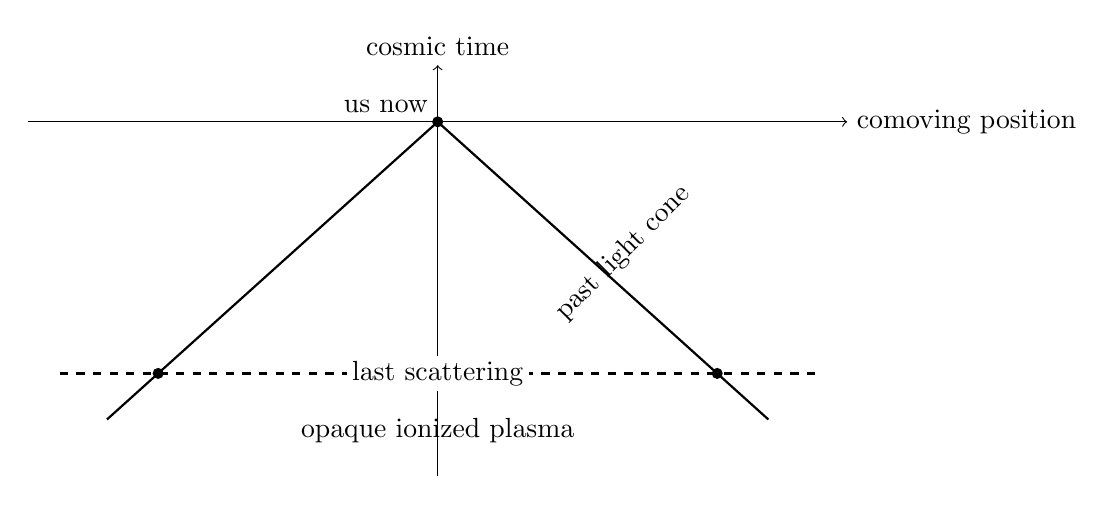
\begin{tikzpicture}[x=1.0cm,y=0.9cm]
\draw[->] (0,0)--(0,5.8) node[above] {cosmic time};
\draw[->] (-5.2,5.0)--(5.2,5.0) node[right] {comoving position};
\draw[thick] (0,5.0)--(-4.2,0.8);
\draw[thick] (0,5.0)--(4.2,0.8);
\draw[thick,dashed] (-4.8,1.45)--(4.8,1.45);
\fill (0,5.0) circle (2pt) node[above left] {us now};
\fill (-3.55,1.45) circle (2pt);
\fill (3.55,1.45) circle (2pt);
\node[fill=white,inner sep=2pt] at (0,1.45) {last scattering};
\node at (0,0.65) {opaque ionized plasma};
\node[rotate=45] at (2.35,3.15) {past light cone};
\end{tikzpicture}
\end{coursefitfigure}
L’observation électromagnétique ne remonte le cône de lumière passé que jusqu’à la surface de dernière diffusion. Avant cette époque, les photons étaient diffusés à plusieurs reprises par le plasma ionisé.\caption{
}
\label{fig:c07-last-scattering}
\end{figure}

\begin{classroomqa}
\audiencequestion{Le découplage met-il fin à toute observation possible des époques antérieures ?}
\lecturerresponse{Il met fin à l’observation directe par voie électromagnétique, car le plasma était opaque aux photons. Des messagers interagissant plus faiblement auraient pu s’échapper plus tôt : en principe, les neutrinos fossiles sondent une couche plus profonde, et le rayonnement gravitationnel peut transmettre des informations d’époques encore plus anciennes. Notre connaissance de l’Univers au-delà de la dernière diffusion est donc en grande partie indirecte, mais elle n’est pas arbitraire. \lecturetimestamp{01:32:27--01:36:31}}
\end{classroomqa}

\begin{classroomqa}
\audiencequestion{Quelle était la valeur absolue de \(a\) au début, et l’Univers était-il nécessairement un objet fini de petite taille ?}
\lecturerresponse{Dans un espace plat, seuls les rapports entre facteurs d’échelle ont une signification invariante ; la normalisation de \(a\) est arbitraire. Une tranche spatiale à courbure négative peut aussi être infinie. Un Univers fermé \(k=+1\) a un rayon de courbure fini, mais les observations déterminent toujours des rapports d’expansion plutôt qu’une taille primordiale connue. Le Big Bang chaud ne signifie pas, à lui seul, que tout l’espace était une petite boule. \lecturetimestamp{01:30:05--01:32:22}}
\end{classroomqa}

\begin{classroomqa}
\audiencequestion{Puisque le fond diffus cosmologique est plus ancien que les galaxies, son observation nous apprend-elle si des galaxies existent aujourd’hui au-delà de notre région observable ?}
\lecturerresponse{Non. Le fond diffus cosmologique montre une région lointaine telle qu’elle était au moment du découplage, et non telle qu’elle est aujourd’hui. La lumière des galaxies actuelles suffisamment éloignées n’a pas encore eu le temps de nous parvenir. Ce qui plaide en faveur de la présence de galaxies au-delà de notre horizon, c’est l’homogénéité observée à grande échelle et l’absence de bord visible, et non une observation directe fournie par le fond diffus cosmologique. \lecturetimestamp{01:59:01--02:00:58}}
\end{classroomqa}

La chronologie ainsi obtenue remonte du présent, en passant par la formation des galaxies et le découplage, jusqu’à l’égalité matière--rayonnement. Plus tôt encore, la diminution du facteur d’échelle implique une hausse de la température et l’apparition de nouvelles espèces de particules.

\section{Égalité matière--rayonnement}

En remontant au-delà du découplage, on rencontre un autre jalon. La matière non relativiste et le rayonnement se diluent différemment :
\begin{equation}
\rho_m\propto a^{-3},
\qquad
\rho_r\propto a^{-4},
\qquad
\frac{\rho_m}{\rho_r}\propto a.
\label{eq:c07-equality-scaling}
\end{equation}
La matière domine à des époques tardives, mais le rayonnement finit nécessairement par dominer lorsque \(a\) est assez petit. La loi d’expansion passe alors du comportement de l’ère dominée par la matière, \(a\propto t^{2/3}\), à celui de l’ère dominée par le rayonnement, \(a\propto t^{1/2}\).

Une estimation délibérément grossière part de \(10^8\) photons par proton, de l’énergie caractéristique \(10^{-4}\,\mathrm{eV}\) d’un photon du fond diffus cosmologique et de l’énergie de masse au repos \(10^9\,\mathrm{eV}\) du proton. En négligeant la matière noire, on obtient
\begin{equation}
\left(\frac{\rho_m}{\rho_r}\right)_0
\sim
\frac{10^9}{10^8\,10^{-4}}
\sim10^5.
\end{equation}
Le raisonnement est ensuite corrigé : la matière noire contribue une masse nettement supérieure à celle des baryons lumineux, ce qui porte l’estimation arrondie à \(10^6\). Dans ce calcul, l’équation~\eqref{eq:c07-equality-scaling} place l’égalité à
\begin{equation}
\frac{a_{\rm eq}}{a_0}\sim10^{-6},
\qquad
\frac{T_{\rm eq}}{T_0}\sim10^6.
\label{eq:c07-equality-estimate}
\end{equation}
Ce sont des estimations de cours destinées à fixer les échelles, et non un ajustement précis des paramètres cosmologiques. Elles montrent comment les puissances différentes de \(a\) situent les ères thermiques successives.

L’ère dominée par le rayonnement se trouve au-delà de la barrière électromagnétique de la dernière diffusion, mais son existence découle des densités mesurées à l’époque récente et des lois d’échelle connues. En remontant vers des températures plus élevées, l’hypothèse selon laquelle les nombres de protons, d’électrons et de photons sont conservés séparément finit par ne plus être valable : les collisions énergétiques commencent à créer des paires particule--antiparticule massives.

\begin{classroomqa}
\audiencequestion{L’affirmation selon laquelle les nombres de photons et de protons sont conservés s’applique-t-elle aussi à la lumière des étoiles et aux températures arbitrairement élevées ?}
\lecturerresponse{Non. Elle s’applique à la population fossile du fond diffus cosmologique pendant l’intervalle où les réactions qui changent le nombre de particules sont inefficaces. La lumière des étoiles est apparue plus tard et est négligeable dans le décompte des photons. À une température assez élevée, la création de paires modifie le contenu en particules et la conservation séparée des nombres cesse d’être valable. La recombinaison elle-même ajoute au plus environ un photon par électron, soit seulement une partie sur \(10^8\) de la population existante du fond diffus cosmologique. \lecturetimestamp{01:26:24--01:27:40}}
\end{classroomqa}

\section{Création de paires et soupe presque symétrique}

À une température de l’ordre de
\begin{equation}
T\sim10^{10}\,\mathrm{K},
\qquad
\frac{a_0}{a}\sim10^{14},
\end{equation}
l’énergie caractéristique des photons est d’environ un mégaélectronvolt, comparable à l’échelle d’énergie de masse au repos nécessaire à la création d’une paire électron--positron. Deux photons peuvent alors réagir selon
\begin{equation}
\gamma+\gamma
\longleftrightarrow
e^-+e^+.
\label{eq:c07-pair-reaction}
\end{equation}
Le seuil exact dépend de la cinématique de la collision, mais l’énergie de masse au repos de l’électron, \(m_ec^2\), fixe l’échelle pertinente.

La création et l’annihilation de paires s’équilibrent rapidement. Si les paires sont trop peu nombreuses, les collisions entre photons en produisent de nouvelles ; si elles sont trop nombreuses, leur annihilation restitue leur énergie aux photons. Les abondances des photons, des électrons et des positrons sont donc déterminées par la température et sont toutes du même ordre dans le plasma relativiste. Elles ne gardent plus de trace simple de leurs nombres ultérieurs.

\begin{classroomqa}
\audiencequestion{Comment ce plasma rempli de paires peut-il rester électriquement neutre s’il y a déjà des électrons qui équilibrent les protons ?}
\lecturerresponse{Chaque réaction crée une charge négative et une charge positive ; les paires n’apportent donc aucune charge nette. Elles forment une population immense et presque symétrique, à laquelle se superpose un minuscule excès d’électrons. Les électrons individuels étant indiscernables, seul l’écart \(N_{e^-}-N_{e^+}\) conserve la charge nécessaire pour équilibrer celle des protons. \lecturetimestamp{01:42:31--01:43:14}}
\end{classroomqa}

Les réactions de création de paires modifient la somme, mais préservent la différence :
\begin{equation}
N_{e^-}+N_{e^+}\quad\hbox{changes},
\qquad
N_{e^-}-N_{e^+}=\hbox{constant}.
\label{eq:c07-pair-invariants}
\end{equation}
Dans la soupe chaude, \(N_{e^-}+N_{e^+}\) est du même ordre que \(N_\gamma\), tandis que l’excès qui subsiste est du même ordre que le nombre, bien plus faible, de protons. On obtient donc le rapport arrondi
\begin{equation}
\boxed{
\frac{N_{e^-}-N_{e^+}}
{N_{e^-}+N_{e^+}}
\sim10^{-8}
}.
\label{eq:c07-asymmetry}
\end{equation}
Il y avait environ un électron excédentaire pour \(10^8\) paires électron--positron.

Cela renverse la question initiale. Le fait remarquable n’est pas simplement que les photons sont nombreux. À haute température, les photons et les paires ont naturellement des abondances comparables. L’énigme est de comprendre pourquoi les populations de particules négatives et positives diffèrent, et pourquoi leur différence relative est infime, plutôt que nulle ou d’ordre un. Un état initial symétrique et une création de paires symétrique ne produiraient aucun excès. L’origine microscopique de l’asymétrie non nulle est le problème que nous aborderons dans la suite.

À des températures encore supérieures de deux ou trois ordres de grandeur, on ne peut plus négliger la structure du proton. Les collisions produisent des quarks et des antiquarks, tandis que les protons se désagrègent en leurs constituants ; photons, leptons, quarks, antiquarks, gluons et espèces sombres assez légères forment un plasma plus chaud. L’énergie du vide y est dynamiquement négligeable, car la densité du rayonnement croît comme \(a^{-4}\).

L’excès de quarks correspondant est lié à l’excès d’électrons par la neutralité électrique globale. Trois quarks de valence forment un baryon ; le décompte fait donc intervenir des facteurs conventionnels, mais la matière baryonique qui subsiste et les électrons qui subsistent ne constituent pas des déséquilibres de charge indépendants. Leur faible abondance commune est un vestige de l’Univers primordial.

Reprenons l’évolution du plasma électron--positron. Lorsque la température passe sous le seuil de production des paires, l’annihilation se poursuit tandis que la réaction inverse devient rare. Presque chaque électron trouve un positron, l’énergie des paires se transforme en rayonnement, et seule subsiste la minuscule population d’électrons sans partenaire. La matière qui nous entoure correspond à ce déséquilibre résiduel, et non à un échantillon représentatif de l’immense population de paires qui existait auparavant.

\begin{classroomqa}
\audiencequestion{Que faisaient les protons pendant l’époque de l’annihilation électron--positron ?}
\lecturerresponse{À cette époque, la température était assez élevée pour créer des paires électron-positron, mais pas encore pour produire en abondance des paires proton--antiproton, ni pour dissoudre les protons en quarks. La population de protons était donc faible, mais persistante, et la neutralité imposait \(N_{e^-}-N_{e^+}\simeq N_p\). \lecturetimestamp{01:55:35--01:56:53}}
\end{classroomqa}

L’Univers visible semble présenter partout le même signe d’excès de matière. L’argument observationnel avancé en cours est l’absence d’antinoyaux dans les rayons cosmiques : des collisions secondaires peuvent produire occasionnellement des antiprotons, mais on s’attendrait à ce qu’une antigalaxie fournisse des antinoyaux complexes. Il s’agit d’un argument observationnel formulé à l’époque du cours, et non de l’affirmation que les régions au-delà de l’horizon observable ont été examinées.

\begin{classroomqa}
\audiencequestion{L’excès de matière observé pourrait-il être une fluctuation locale, avec des régions d’antimatière au-delà de ce que nous pouvons voir ?}
\lecturerresponse{Le fait que le signe soit le même dans l’immense volume observable est beaucoup trop cohérent pour s’expliquer par une fluctuation aléatoire. Il faut une explication dynamique. Au-delà de la région observable, toutefois, nous ne disposons pas de preuves directes ; on ne peut exclure une transition vers un domaine différent au seul motif qu’on regarde plus loin que la lumière n’a pu nous parvenir. \lecturetimestamp{01:56:57--01:58:47}}
\end{classroomqa}

\begin{classroomqa}
\audiencequestion{L’explication matière--antimatière constitue-t-elle déjà une théorie numérique précise, et l’unification des forces a-t-elle lieu à cette température ?}
\lecturerresponse{Il existe une théorie qualitative de la façon dont une faible asymétrie peut apparaître, mais la valeur arrondie \(10^{-8}\) n’est pas déduite ici d’un modèle microscopique unique. L’unification des forces relève de températures bien supérieures à celles de l’époque des paires électron-positron. Ces deux questions nécessitent une physique qui dépasse les jalons thermiques abordés ici. \lecturetimestamp{01:51:36--01:52:24}}
\end{classroomqa}

\section{À retenir}

L’histoire thermique est structurée par les taux et les seuils. Les diffusions rapides établissent une température commune ; la formation des atomes neutres supprime les diffuseurs ; l’expansion uniforme décale alors vers le rouge un spectre de Planck figé, sans en déformer la forme. Le fond diffus cosmologique est donc à la fois un thermomètre du rayonnement et une surface visible qui marque la fin de l’accès électromagnétique direct au plasma antérieur.

L’excès de photons fait de la recombinaison un problème de queue de distribution, plutôt qu’un problème d’énergie moyenne. L’échelle \(T_{\rm dec}/T_0\sim10^3\) situe la dernière diffusion, tandis que les lois de dilution différentes de la matière et du rayonnement situent une époque d’égalité antérieure. À des températures encore plus élevées, la création de paires efface la mémoire des nombres totaux d’électrons et de positrons, mais préserve leur infime différence. Cette asymétrie résiduelle, reflétée dans le secteur baryonique, est la donnée initiale inexpliquée à laquelle la prochaine étude devra s’attaquer.